\documentclass[border=0]{standalone}
\usepackage[T1]{fontenc}
\usepackage{lmodern}

\usepackage{tikz}
\usetikzlibrary{calc}
\begin{document}%
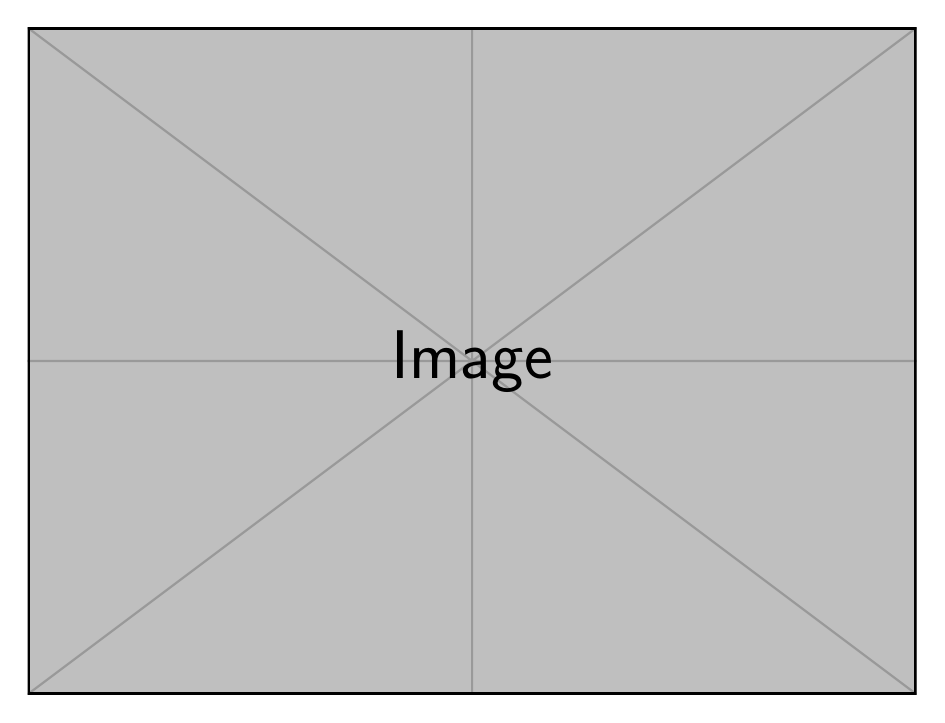
\begin{tikzpicture}[x=32bp,y=24bp]% 4x3
    \clip (0,0) rectangle (10,10);
    \path [fill=black!25] (0,0) rectangle (10,10);
    \draw [thick,black!40]
        (0,0) -- (10,10)
        (10,0) -- (0,10)
        (5,0) -- (5,10)
        (0,5) -- (10,5)
    ;
    \path [draw,ultra thick] (0,0) rectangle (10,10);
    \path let \p1=(2,0), \p2=(2.4,0), \p3=(.4,0), \p4 = (.48,0) in
       node at (5,5) {\sffamily\fontsize{\x1}{\x2}\selectfont Image}
    ;
\end{tikzpicture}%
\end{document}%
